
\chapter{State of the art}
\label{chapter:state}

Being a large domain, deep learning imposes a research in multiple subdomains such as neuroscience, reinforcement learning, neural networks or convolutional neural networks. That being said, this chapter is dedicated to gathering information on each of them.

\section{Reinforcement learning}
\label{sec:reinforcement}

\subsection{History}
The history of reinforcement learning starts with the pavlovian experiment\cite{pavlov} in 1903, when Pavlov tried to demonstrate that there is a connection between conditioned and unconditioned stimulus. The unconditioned response of salivation of a dog is fired up by bringing an unconditioned stimulus as food. If we try to make the dog to salivate in the presence of a neutral stimulus(the sound of a bell) we won't succeed, but if we use in the same time the unconditioned and neutral stimulus we can make the dog salivate and transform the bell and salivation in conditioned stimulus and conditioned response.

\subsection{Q-Learning. Sarsa}
\label{qlearning-sarsa}

\subsubsection{Q-Learning}
\label{qlearning}
Q-Learning\cite{norvig} is the algorithm for learning in small steps details about the environment. We know the initial starting state of the game and also a set of possible actions we can take in order to change the current state. At the beginning, we are constrained to choose randomly an action, because we do not know which one could bring us winning the game and this is the exploration phase. We keep randomly picking actions until the game is finished.

A game can have \textbf{n} number of states and \textbf{a} number of actions. We keep in memory a table \textbf{Q} of size \textbf{nxa} and we initialize all the corresponding elements with zero. During the game, rewards can be granted. Some of them can be good rewards and some of them can be bad rewards. When we recieve rewards, we update the previous state with the score obtained.

Here we have to choose between exploration and exploitation. In the first states of the game, when we know nothing about environment, so we choose to explore new states in order to see if they bring us rewards. After some \textbf{e} episodes we learn which actions can bring us closer to the winning of the game. This is the moment when to start to exploit the things we have already learnt in the previous episodes. Assume we are in state \textbf{s} and have the next possible actions \{$a_{1},a_{2},a_{3},a_{4}$\}. Keep in mind that we recorded the Q-table. At this moment we choose the action which gives us the best utility from states s. If \textbf{Q(s,$a_{3}$)} is the maxim value of \textbf{Q} in state \textbf{s} we will pick action \textbf{$a_{3}$}.

\subsubsection{Sarsa}
\label{sarsa}
Q-Learning and Sarsa look alike except for the fact that Sarsa is updating his policy based on the action it takes and which is not necessary the best action, but it is the action expected to pursue his policy.


When dealing with large negative rewards Q-Learning is dealing better than Sarsa\cite{multi-agent} because Q-Learning does not avoid risk situations while Sarsa is avoiding them. Both algorithms have variables that have to be adjusted during the computation.

\begin{itemize}
  \item \textbf{Learning rate} adjusts learning of new information flow. \textbf{0} is for not acquiring information and \textbf{1} is for considering only the new information.
  \item \textbf{Discount factor} adjust the importance of current rewards(\textbf{1}) vs future rewards(\textbf{0})
\end{itemize}

$\epsilon$-Greedy is the policy for choosing the next action. As we have already mentioned the problem between choosing explorations vs. exploitation, this strategy comes for helping in the first episodes where we don't have too much details about environment. It says that we can choose randomly an action from the set of actions with probability $\epsilon$ and choose the best action with probability $1-\epsilon$.

Figure \ref{fig:svsq} shows behaviour of Q-Learning and Sarsa 

\begin{figure}[h]
	\begin{center}
		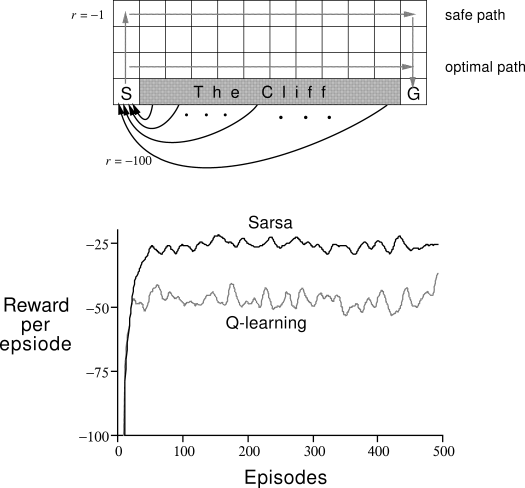
\includegraphics[width=282px,height=288px]{src/img/state/qsrewards}
		\caption{Q-Learning vs Sarsa\cite{sutton}} \label{fig:svsq}
    \end{center}
\end{figure}


\section{Neural Networks and Convolutional Neural Networks}

In this chapter we will discuss how networks works, the principles behind them and what optimization techniques we can use. It is worth mentioning that the information is splitted in data, model, loss functions, train and test.
\begin{figure}[h]
	\begin{center}
		\includegraphics[width=294px,height=186px]{src/img/state/nn2}
		\caption{example of neural network} \label{fig:nn}
    \end{center}
\end{figure}

\subsection{Data}
\label{data}
The data resulted from pre-processing step is crucial for learning. To differentiate between noisy images and/or bad lighting is a big problem for a network because it may learn the inappropriate features.

One of the first concerns is choosing the color space. We can have RGB(Red Green Blue) or we can have YUV(luminance blue–luminance red–luminance). In many cases RGB is the first choice instead of YUV\cite{pipeline}. If we are interested in color both of them are a good choice, but if we are intrested in edges the luminance channel it will be more suitable.

\begin{figure}[h]
	\begin{center}
		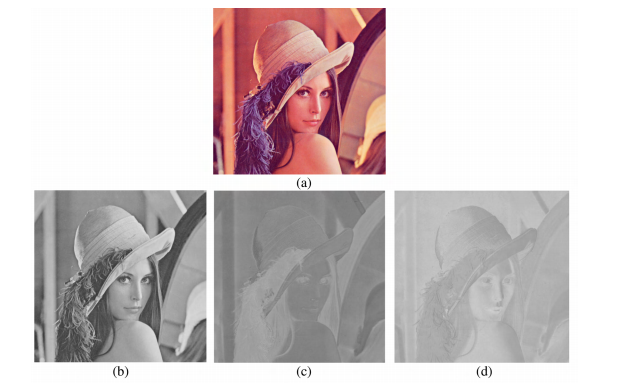
\includegraphics[width=410px,height=102px]{src/img/state/lenayuv}
		\caption{Lena: RGB and Y, U, V channels} \label{fig:lenayuv}
    \end{center}
\end{figure}

If values have different ranges of scales, then logarithmic normalization should be used. In distance-based classification, if we have a feature with values between [0, 1] and another feature with values between [0, 2000] we need to normalize the data between [0, 1] or [-1, 1] such that every variation of each feature counts the same as the other feature. We do not want to start with giving more importance to a feature than the others.

Another aspect that should be considered is the importance of illumination conditions. If we are not interested than we remove the mean-value for each samples. If we have thousand of pictures with different illumination condition we remove the average illumination by extracting the mean-value such that all the pictures have the same contrast.

Splitting data is another importan aspect in training networks. We have to have three sets: train sets, test sets and validation sets. 50\% of initial data goes to training and the rest fifteen percent is splitted in 25\% for testing and 25\% for validation. This is used when the dataset is very large. Having a small dataset implies the statretgy to split data into $\frac{2}{3}$ for training and $\frac{1}{3}$ for testing\cite{splitting}.


Cross validation\cite{cross-validation} should also be also taken into consideration. Cross validation is the algorithm of splittng data into test dataset and train dataset forcing both sets cross-over in succesive epochs such that every part in the initial dataset validates the model of the neural network. Assume that we have splitted data into \{\textbf{A}, \textbf{B}, \textbf{C}\}, each one being $\frac{1}{3}$ of initial dataset. In the first iteration we take the model to train on \textbf{A} and \textbf{B} and test it with \textbf{C}. The second iteration implies the training on \textbf{A} and \textbf{C} and testing on \textbf{B} and the last iteration implies training on \textbf{B} and \textbf{C} and testing on \textbf{A}. In this way we can assure that our model is working well for every case.



\subsection{Model}
\label{model}

%------------------------Nonlinear activation functions------------------------

\subsubsection{Nonlinear activation functions\cite{david,hiddenfunctions,backprop}}
\label{transfer}
Activation functions are used to define a connection between input and output.

\textbf{Hyperbolic tangent function(tanh)}
\begin{itemize}
	\item outputs values between 0 and 1
	\item outputs are zero-centred
	\item if extremely large negative numbers are given as input, the output will be close to -1 and the error will propagate correctly
	\item generally used in hidden layers
	\item tanh layers learn fasten than sigmoid layers because of the size of the gradient
\end{itemize}

\begin{figure}[h]
	\begin{center}
		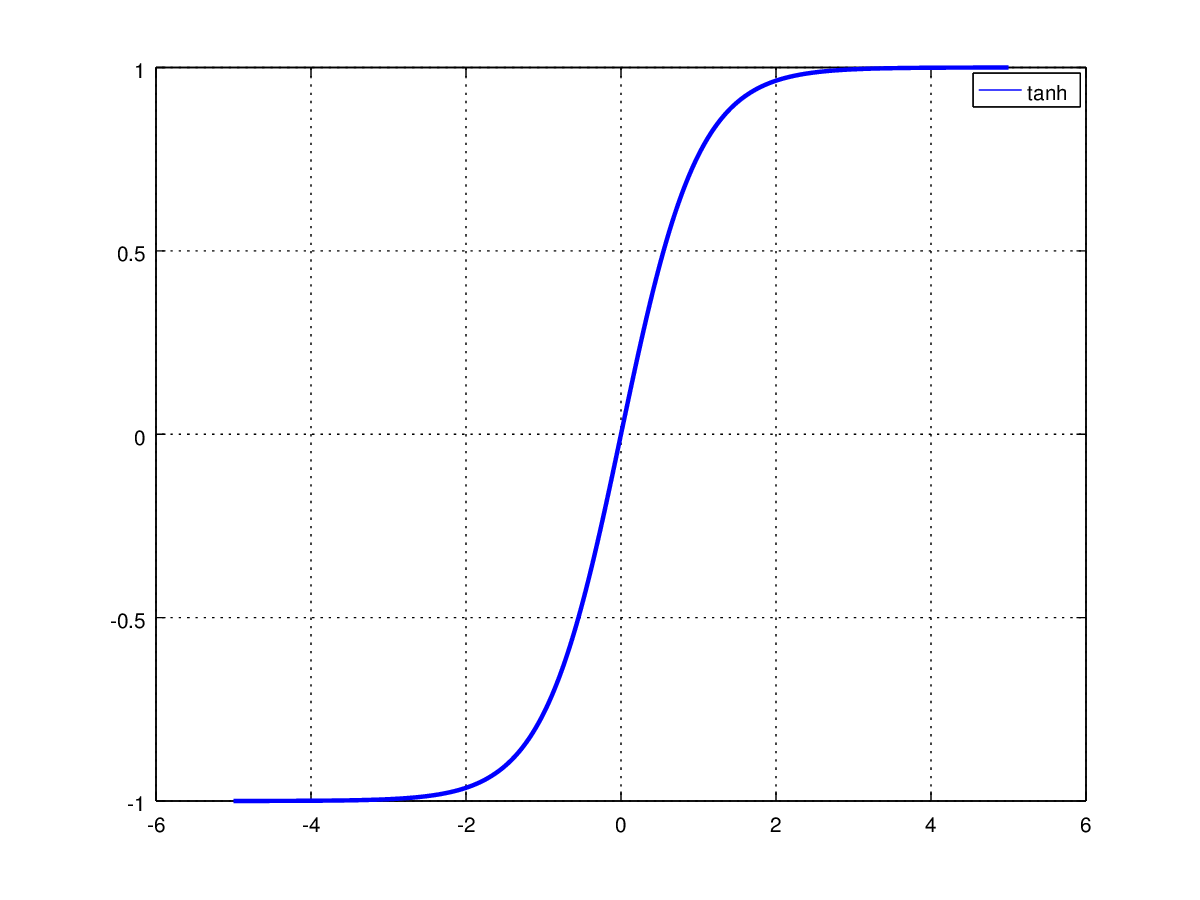
\includegraphics[width=240px,height=180px]{src/img/state/tanh}
		\caption{tanh function} \label{fig:tanh}
    \end{center}
\end{figure}


\textbf{Sigmoid function(sigmoid)}
\begin{itemize}
  \item learning values far away from threshold is difficult
  \item useful for backpropagation algorithms
  \item easy for calculating derivatives and used in gradient descent methods
  \item output values between 0 and 1
  \item can be used in binary classification problems with setting some threshold
  \item if extremely large negative numbers are given as input, the output will be close to zero and the error will not propagate correctly
\end{itemize}

\begin{figure}[h]
	\begin{center}
		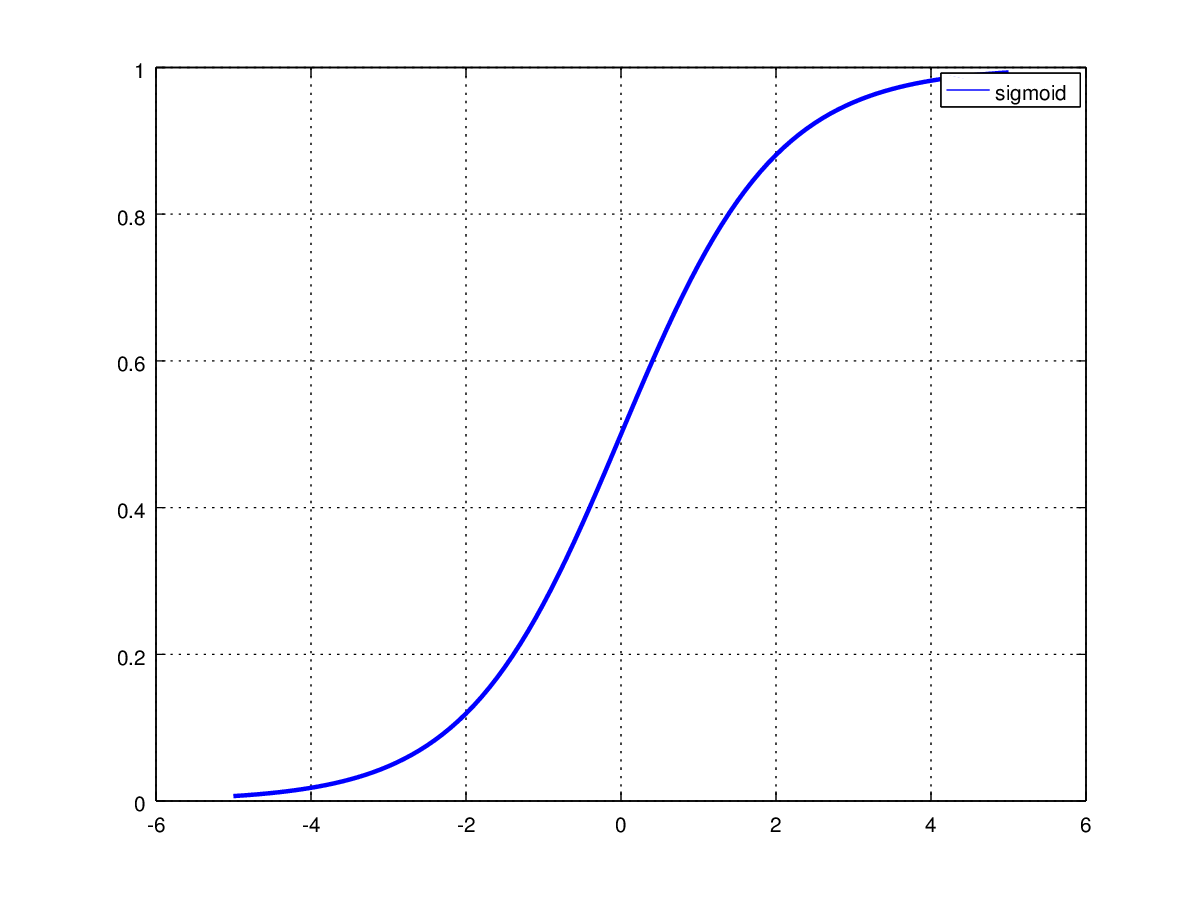
\includegraphics[width=240px,height=180px]{src/img/state/sigmoid}
		\caption{sigmoid function} \label{fig:sigmoid}
    \end{center}
\end{figure}

\textbf{Rectified Linear Units(ReLU)}
\begin{itemize}
	\item better results in networks combined with stochastic gradient descent than tanh/sigmoid\cite{imagenet}
	\item ReLU is determined to be better than tanh/sigmoid empirically
\end{itemize}

\begin{figure}[h]
	\begin{center}
		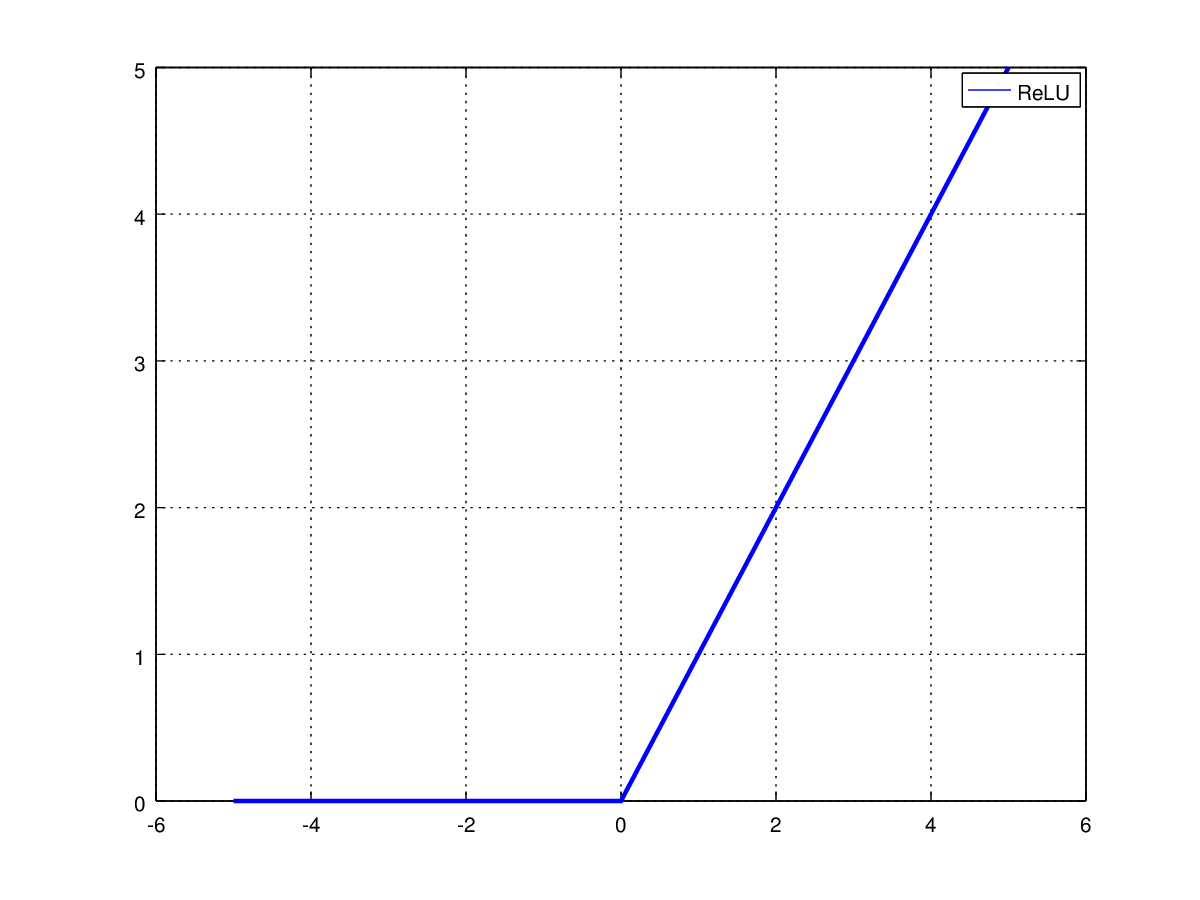
\includegraphics[width=240px,height=180px]{src/img/state/relu}
		\caption{ReLU} \label{fig:relu}
    \end{center}
\end{figure}

%------------------------Convolutional layers------------------------
\newpage
\subsubsection{Convolutional layers}
Pooling layers can be used in getting rid of unwanted information and also can be useful in dimensionality reduction.

\textbf{Spatial Convolution}
\begin{itemize}
	\item{used to modify the frequency of neighbourhood pixels}
	\item{accentuates edges in combination with Gabor filters}
	\item{can be used to obtain gaussian blur effect}
	\item{suppose we have an image of \textbf{width x height} size, if we apply a convolutional kernel of size \textbf{kw x kh} the size of the output will become \textbf{(width - kw + 1) x (height - kh + 1)}}
\end{itemize}


\begin{figure}[h]
	\begin{center}
		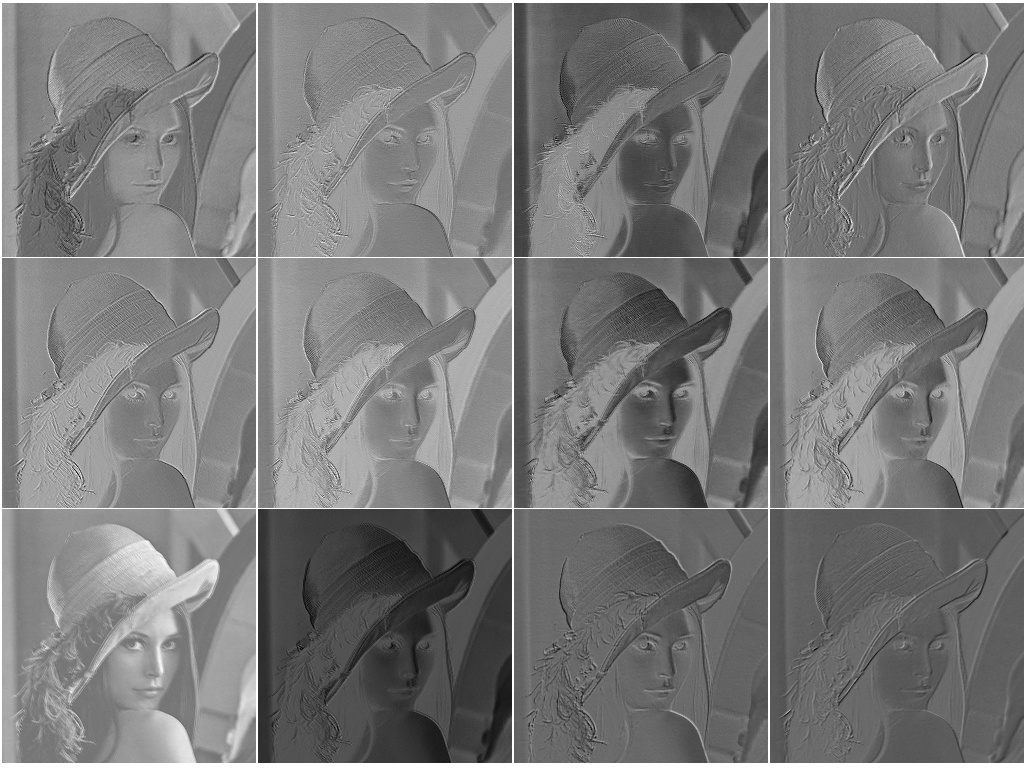
\includegraphics[width=240px,height=180px]{src/img/state/lena-spatialconv22}
		\caption{Spatial Convolution(2D) with 12 output channels, 5x5 kernel matrix and 2x2 stride} \label{fig:lena-spatialconv}
    \end{center}
\end{figure}

\begin{figure}[h]
	\begin{center}
		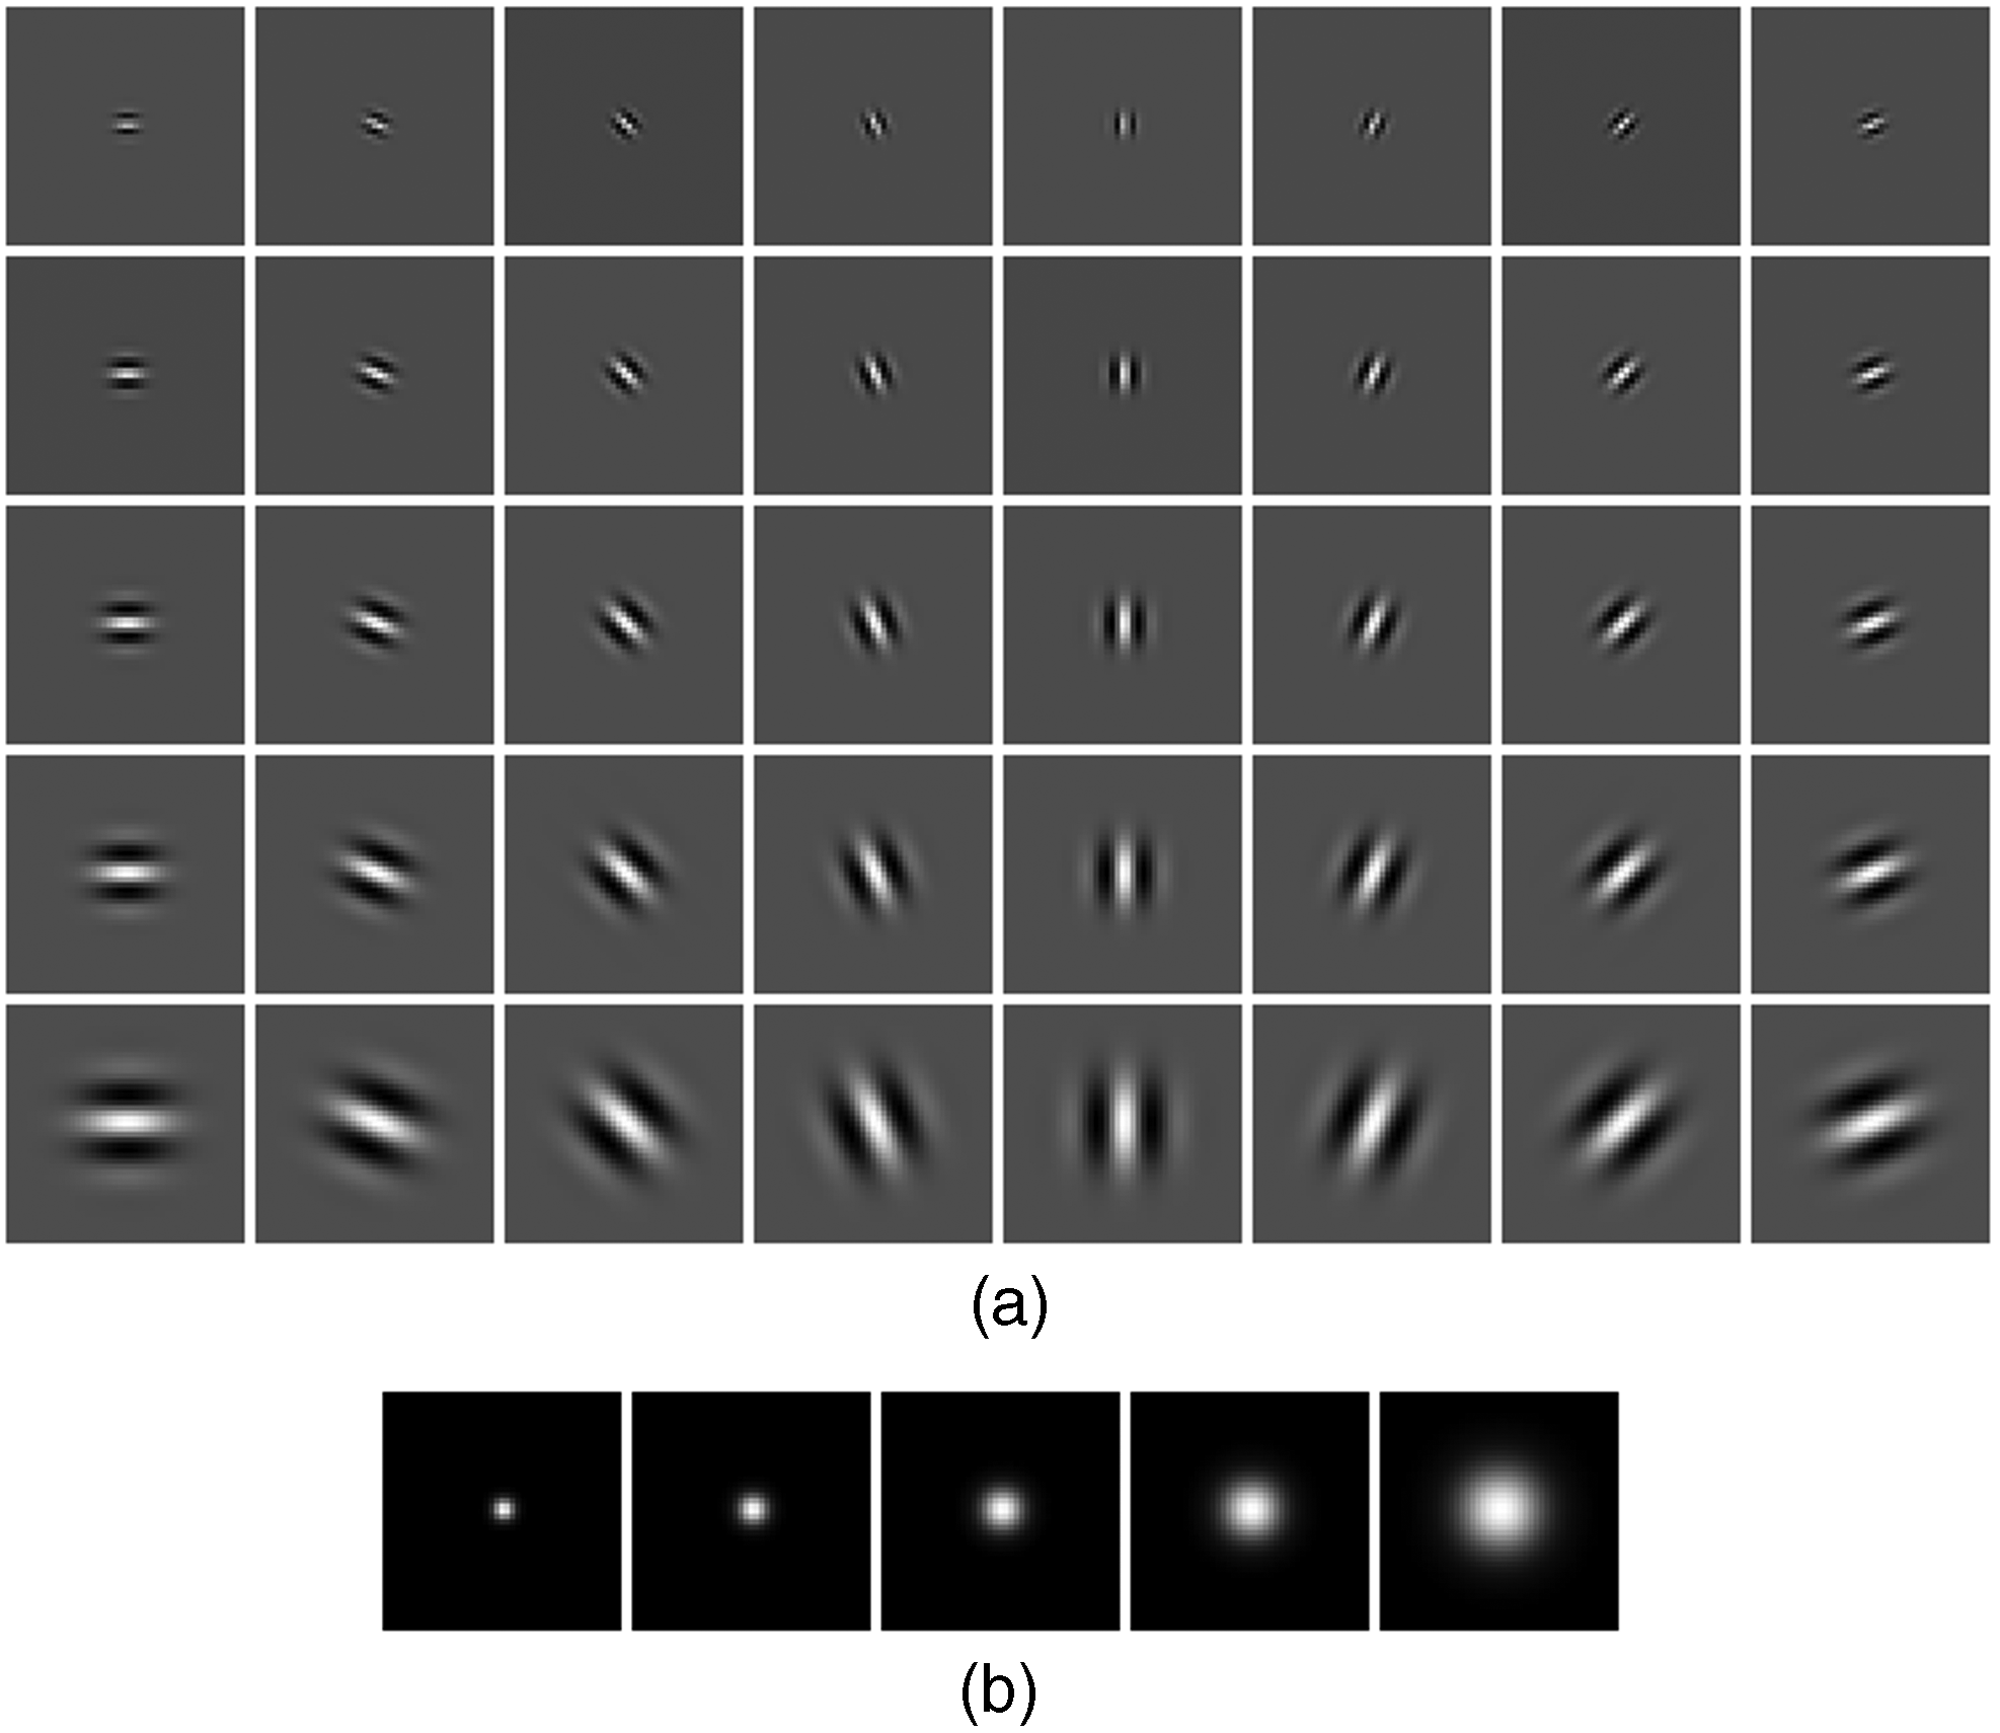
\includegraphics[width=240px,height=180px]{src/img/state/gabor}
		\caption{Gabor filters\cite{gabor}} \label{fig:gabor.png}
    \end{center}
\end{figure}

\newpage
\textbf{Average pooling}
\begin{itemize}
	\item{useful for dimensionality reduction}
	\item{acts poorly in some situations as opposed to max-pooling}
\end{itemize}
\begin{figure}[h]
	\begin{center}
		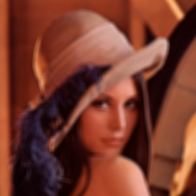
\includegraphics[width=140px,height=140px]{src/img/state/lena-avgpooling}
		\caption{Average pooling with 10x10 kernel matrix and 2x2 stride} \label{fig:lena-avgpooling}
    \end{center}
\end{figure}



\textbf{Max pooling}

\begin{itemize}
	\item{useful for dimensionality reduction}
	\item{useful for activating features that have a low probability of being activated\cite{maxpooling}}
	\item{if a feature appears in a cell it is less probably to appear in the neighbourhood cells}
\end{itemize}

\begin{figure}[h]
	\begin{center}
		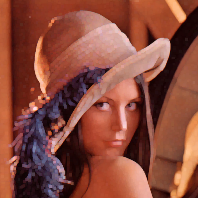
\includegraphics[width=140px,height=140px]{src/img/state/lena-maxpooling}
		\caption{Max pooling with 5x5 kernel matrix and 2x2 stride} \label{fig:lena-avgpooling}
    \end{center}
\end{figure}


\newpage
\subsection{Loss functions}
\label{loss}

Loss functions are used to aproximate how far we are from the solution, the diffrence between observed values and predicted values.

\textbf{Mean squared error}
\begin{itemize}
	\item{useful for regression}
	\item{not used in classification problems}
\end{itemize}
\begin{equation}
J(weights) = \frac{1}{2\cdot no_{samples}}\cdot\displaystyle\sum_{i=1}^{no_{samples}}\cdot(nn_{weights}(samples^{(i)}) - labels^{(i)})^2
\end{equation}

\textbf{Hinge loss (margin criterion)}
\begin{itemize}
	\item{useful for binary classifications}
	\item{forces labels to be -1 or 1}
\end{itemize}
\begin{equation}
J(weights) = \displaystyle\sum_{i=1}^{no_{samples}}max(0, 1 - labels^{(i)}\cdot nn_{weights}(samples^{(i)}))
\end{equation}


\subsection{Optimizations for learning\cite{ng}}
Optimization algorithm are used in updating the weights in a neural network in concordance with a loss function.
\label{optimization}
Assuming that our cost function is defined as follows:
\begin{equation}
	J(weights_n) = \frac{1}{2no_{samples}}\cdot\displaystyle\sum_{i=1}^{no_{samples}}(nn_{weights}(samples^{(i)}) - labels^{(i)})^2
\end{equation}
we state that derivative of \textbf{J} w.r.t \textbf{weights} is:
\begin{equation}
	\frac{\partial J}{\partial weights} = \frac{1}{no_{samples}}\cdot\displaystyle\sum_{i=1}^{no_{samples}}(nn_{weights}(samples^{(i)}) - labels^{(i)})
\end{equation}
Updating weights is done in accordance with the derivative of cost function.
\begin{equation}
	weights_n = weights_n - \alpha\cdot\frac{\partial J}{\partial weights}
\end{equation}
where $\alpha$ represents learning rate.

\newpage
\textbf{Gradient descent (GD)}

\begin{itemize}
	\item{if $\alpha$ is too small, GD converges slow}
	\item{if $\alpha$ is too large, GD can converge to local minimum and not global minimum}
	\item{recommended for huge number of samples}
	\item{require more iterations than SGD}
\end{itemize}

\begin{algorithm}
	\floatname{algorithm}{Algorithm}
	\caption{Gradient Descent} \label{gd-code}
	\begin{algorithmic}[1]
		\Repeat
       			\For{\texttt{j = 1, no_weights}}
       				\begin{equation}
					weights_j = weights_j - \alpha\displaystyle\sum_{i=1}^{no_{samples}}(nn_{weights}(samples^{(i)}) - labels^{(i)})\cdot {samples_j}^{(i)}
					\end{equation}
      			\EndFor
		\Until{convergence is obtained}
	\end{algorithmic}
\end{algorithm}


\vspace{8mm}


\textbf{Stochastic gradient descent (SGD)}

\begin{itemize}
	\item{very fast is number of samples is small}
	\item{iterations are removed by computing $(X^T\cdot X)^{-1}$}
	\item{requires regularization}
	\item{needs feature scaling}
\end{itemize}

\begin{algorithm}
	\floatname{algorithm}{Algorithm}
	\caption{Stochastic Gradient Descent} \label{sgd-code}
	\begin{algorithmic}[1]
		\Repeat
			\State shuffle dataset (randomly)
			\For{\texttt{i = 1, no_samples}}
       			\For{\texttt{j = 1, no_weights}}
       				\begin{equation}
					weights_j = weights_j - \alpha\cdot(nn_{weights}(samples^{(i)}) - labels^{(i)})\cdot {samples_j}^{(i)}
					\end{equation}
      			\EndFor
      		\EndFor
		\Until{convergence is obtained}
	\end{algorithmic}
\end{algorithm}

\newpage

\subsection{Training and testing}
\label{train-test}

The question now arises: when do we have to stop with training if a (convolutiona) neural network ?
We have to take care of how much we train a network. If we train too much, it will learn the samples and will predict exactly the same values, but there will be a large error for samples it has not seen. If we train too little, the network will not learn how to predict the samples it has seen and will also have a large test error.
Mathematically, the moment when we should stop with training is the moment when the test error will increase its value. In \ref{fig:traintest} we can see the optimum moment when we should stop training.

\begin{figure}[h]
	\begin{center}
		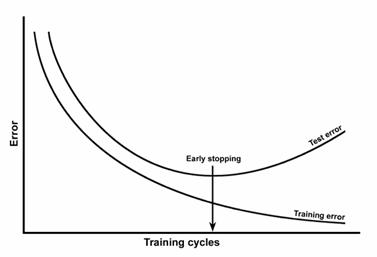
\includegraphics[width=188px,height=129px]{src/img/state/traintest}
		\caption{train-test error\cite{traintest}} \label{fig:traintest}
    \end{center}
\end{figure}

Underfitting means also high bias and represents the incapacity of the algorithm to recognize the pattern feaures in samples.

Overfitting means also high variance and represent the incapacity of the algorith to adapt to new samples.

Both of them are illustrated in the figure \ref{fig:overfitting}.

\begin{figure}[h]
	\begin{center}
		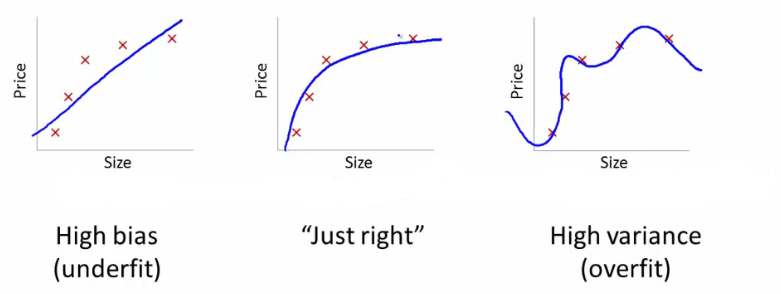
\includegraphics[width=390px,height=147px]{src/img/state/overfitting}
		\caption{underfitting, bias-variance trade-off and overfitting\cite{ng}} \label{fig:overfitting}
    \end{center}
\end{figure}

\newpage

\section{An in-depth look to ``Playing Atari with Deep Reinforcement Learning'' and paper\cite{atari}}
This section is dedicated to analyzing the paper in which is proposed the method to solve playing games using deep learning and reinforcement learning.

\subsection{Architecture\cite{nature}}
The article ``Human-level control through deep reinforcement learning'' proposes a new type of network, Q-network which combines convolutional layers, a representation of human receptive fields and pooling layers used for dimensionality reduction. The input layer is represented by \textbf{84x84x4} neurons for the image produced after preprocessing frames from the game and is followed by three convolutional layers, two fully connected layer and the output layer which has a number of neurons equal with the number of actions corresponding to each game. Each hidden layer is followed by a rectified linear unit (ReLU).

\begin{figure}[h]
	\floatname{algorithm}{Algorithm}
	\begin{center}
		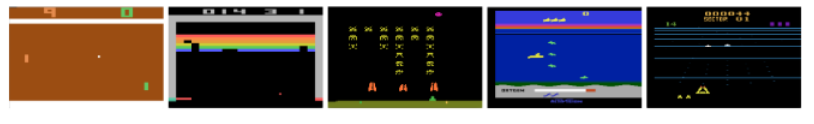
\includegraphics[width=380px,height=58px]{src/img/state/ataripic}
		\caption{Snapshots with five Atari 2600 Games: Pong, Breakout, Space Invaders, Seaquest, Beam Rider} \label{fig:ataripic}
    \end{center}
\end{figure}




\begin{figure}[h]
	\floatname{algorithm}{Algorithm}
	\begin{center}
		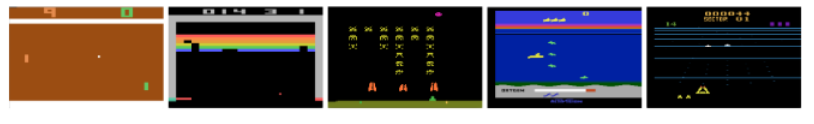
\includegraphics[width=380px,height=58px]{src/img/state/ataripic}
		\caption{Snapshots with five Atari 2600 Games: Pong, Breakout, Space Invaders, Seaquest, Beam Rider} \label{fig:ataripic}
    \end{center}
\end{figure}